
	\begin{tcolorbox}[colback=blue!5!white,colframe=blue!75!black,title=Definición]

	Los motores eléctricos son máquinas que transforman la energía eléctrica en movimiento (energía cinética). Estos aparatos se componen, básicamente, del rotor y de un estator donde tiene bobinas inductoras desfasadas entre sí 120°\end{tcolorbox}

		
	

\subsubsection{Especificaciones}

	El motor (Figura \ref{fig:motor}) asincrónico que se utiliza es de la marca \textbf{Altium} perteneciente a la firma \textbf{Schneider Electric}. Las especificaciones se muestran a continuación \\
	\paragraph*{Altium Eff2}
	
\begin{minipage}[t]{.5\textwidth}
	\begin{itemize}
		\item Tipo: TE2A90SP2
		\item Tensión nominal: 220/380 V
		\item Corriente nominal: 5.97 A 
		\item Frecuencia nominal:  50 Hz.
		\item Potencia: 1.5kW / 2 HP
		\item Fases: 3
		\item Factor de Potencia: 0.84
	\end{itemize}
\end{minipage}	
\begin{minipage}[t]{.5\textwidth}
	\centering\raisebox{\dimexpr \topskip-\height}{%
	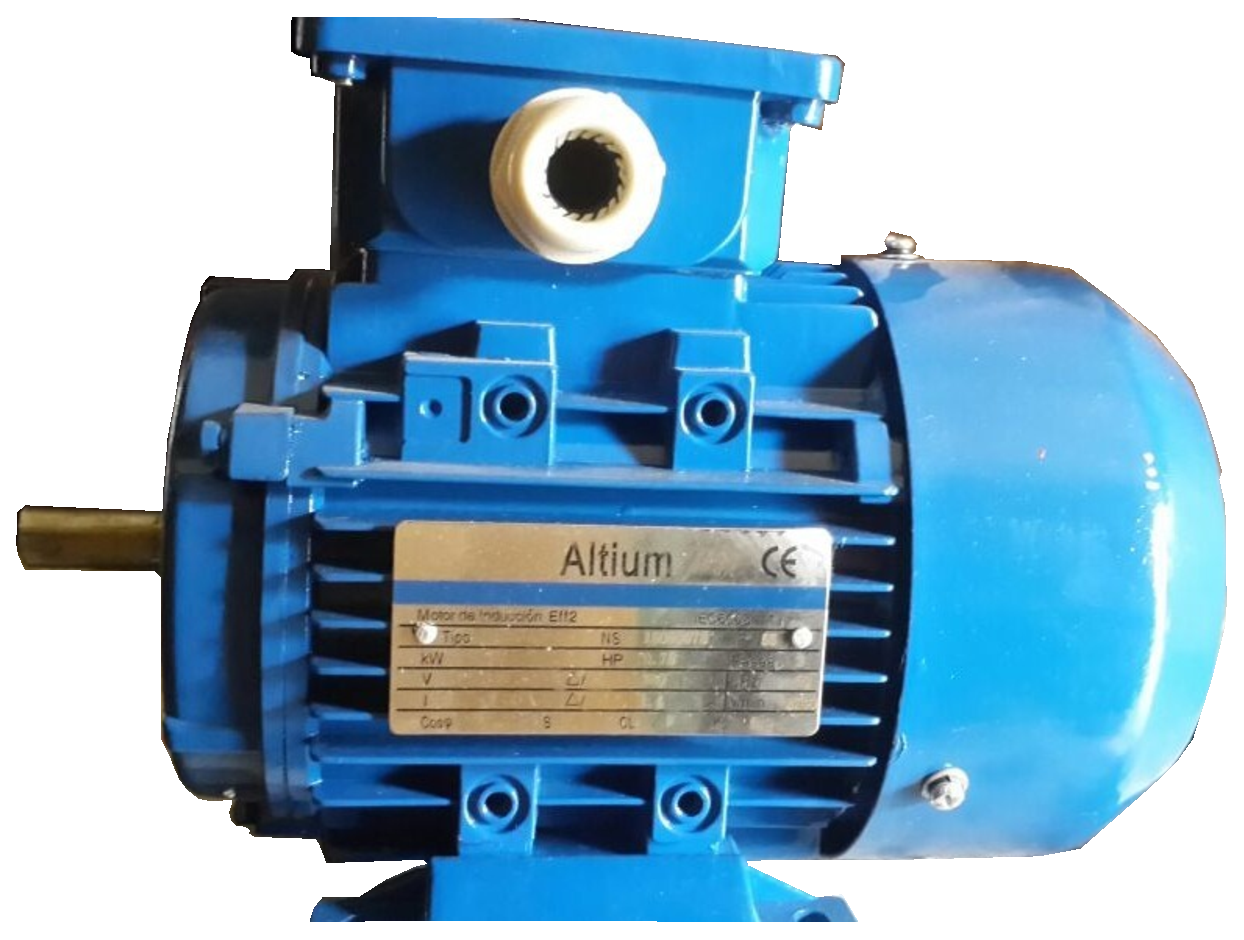
\includegraphics[scale=0.3]{motor.eps}}
	\captionof{figure}{Motor Altium}
	\label{fig:motor}

 \end{minipage}
	\newpage